\chapter{Proposta para análise de arquiteturas de microsserviços \ac{mmorpg}}
\label{cap3}

Para realizar a análise de consumo de recursos de uma arquitetura de jogos \ac{mmorpg} é necessário coletar / medir os recursos utilizados para posterior análise.
%
Na fase de coleta de informação, é possível utilizar ferramentas existentes para coletar informações sobre o consumo da rede (\textit{e.g.}, Tcpdump, Wireshark, etc.) e consumo de recursos computacionais do serviço (e.g., Golang Flame, Ruby Thread profiler tool, Golang profiler, \textit{etc.})
%
Estas ferramentas contribuem com a análise, sendo de extrema importância para a coleta de dados.



Contudo, se faz necessário uma arquitetura de microsserviços para jogos \ac{mmorpg} a fim de ser utilizado para análise.
%
Esta arquitetura será descrita na Seção~\ref{sec:arquitetura_proposta}.



\section{Arquitetura proposta para análise}
\label{sec:arquitetura_proposta}

Esta seção tem como objetivo descrever a arquitetura implementada para análise, baseada na arquitetura Salz~\cite{albion_online_unite}.
%
A mesma arquitetura é utilizada no jogo Sandbox-Interactive Albion\footnote{Sandbox-Interactive Albion: \url{https://albiononline.com/en/home}}.
%
Ela pode ser vista em uma visão macro na Figura~\ref{fig:salz}.


\begin{figure}[htb!]
\caption{Arquitetura de microsserviços proposta para análise.}
\label{fig:salz}
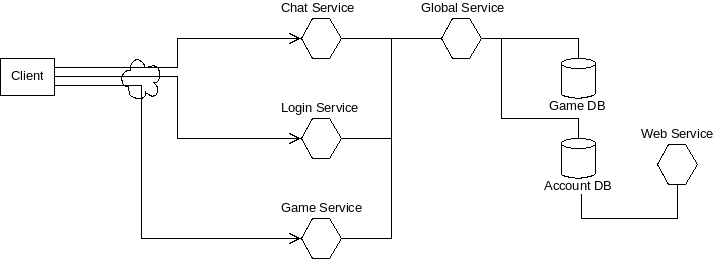
\includegraphics[height=5cm]{img/cap3/salz.png}
\centering

Adaptado de:~\cite{albion_online_unite}.
\end{figure}



Essa arquitetura contém os seguintes microsserviços:

\begin{itemize}
  \item \textbf{Login Service}: Responsável por gerenciar as conexões do jogo e fornecer autorização aos clientes para os demais microsserviços.
  \item \textbf{Chat Service}: Receberá mensagens e distribuirá aos demais jogadores da mesma região ou enviará mensagens diretas a outros jogadores. Ele receberá a conexão diretamente do jogador, e por sua vez será necessário utilizar o \textit{Login Service} para autenticar a conexão.
  \item \textbf{Game Service}: Gerenciará um pedaço do ambiente do jogo. Cada microsserviço desta categoria será responsável por um pedaço do jogo, controlando as ações dos personagens em relação a sua área de interesse. Ele receberá a conexão diretamente do cliente, e por sua vez precisa utilizar o \textit{Login Service} para autenticar a conexão.
  \item \textbf{Global Service}: Este microsserviço resolve as requisições globais requisitadas pelo \textit{chat service}, \textit{login service} ou \textit{game service}.
  \item \textbf{Web Service}: Servirá para gerência de contas pessoais, autenticação e afins.
  \item \textbf{Game DB}: Banco de dados em memória utilizado pelos microsserviços.
  \item \textbf{Account DB}: Banco de dados persistente.
\end{itemize}


Para melhor compreendimento se faz necessário a descrição específica de funcionamento em cada microsserviço, tecnologias e protocolos utilizados e esquema de funcionamento.
%
Além disso será obrigatório descrever os microsserviços de GameDB e AccountDB utilizados na arquitetura.

\subsection{Login Service}

Microsserviço respoonsável por efetuar a autenticação do usuário ao mundo.
%
Ele será responsável por impedir multiplas conexões utilizando um mesmo usuário.



Além dessa funcionalidade, outro objetivo deste microsserviço é descrever o status de conexão de um jogador, a fim de sinalizar os demais microsserviços que o mesmo desconectou do serviço.
%
Ele será o responsável pela descrição de status da atual conexão do jogador com o serviço visto que os demais microsserviços estão trabalhando de forma isolada.
%
Isto servirá para evitar requisições maliciosas ao serviço.



Este microsserviço usará Redis, um banco NoSQL baseado em chave-valor de armazenamento em memória para armazenar tokens de autenticação de uma conexão.
%
Para gerar este token, será utilizado a tecnologia \ac{jwt}.

\subsection{Chat Service}


Este microsserviço será responsável por redirecionar mensagens a jogadores.
%
Ele terá duas principais funções:

\begin{itemize}
  \item Enviar mensagens aos personagens que estão na área de interesse do remetente.
  \item Enviar mensagens diretas a outros personagens.
\end{itemize}


\subsection{Game Service}

Este microsserviço gerenciará conexões de uma determinada região do ambiente do jogo, nomeado \textit{chunk}.
%
Ele servirá para atualizar a árvore de cena do cliente e executar operações sobre a árvore de cena do chunk a qual o serviço ficou responsável.
%
A abordagem de divisão em \textit{chunks} serve para minimizar a influência de conexões sobre as operações no mundo, e assim permitir mais conexões sobre o mundo como um todo.
%
Entretando é necessário todar uma abordagem para definir a troca de contexto entre duas \textit{chunks} no jogo.
%
Neste microsserviço foi escolhida a abordagem sobre banco de dados, onde o jogador terá que informar a troca de mapa e armazenar estra troca de dados no banco para que o microsserviço que controla esta região possa resgatar seus dados e prosseguir com o jogo.



\subsection{Global Service}

Este microsserviço realizará o meio de campo entre todos os microsserviços.
%
Ele será responsável por sincronizar as posições dos personagens entre o Chat Service e Game Service, atualizar informações do GameService no AccountDB além de gerenciar o GameDB.
%
Ele é uma aplicação \textit{Web} e pode ser um gargalo na aplicação.

\subsection{Web Service}

Este microsserviço será responsável por exibir dados do banco aos jogadores.
%
No contexto de simulação ele servirá para realizar operações \ac{crud} manuais e automatizadas no banco, além de gerenciar migrações no mesmo.

\subsection{GameDB}

\subsection{AccountDB}
